\newcommand{\Fab}{F^{\alp \bet}}
\newcommand{\Ua}{U^\alp}
\newcommand{\Usa}{U_\alp}
\newcommand{\Ub}{U^\bet}
\newcommand{\Xa}{X^\alp}
\newcommand{\Xsa}{X_\alp}
\newcommand{\Xb}{X^\bet}
\newcommand{\xap}{x^\alp_p}
\newcommand{\xaq}{x^\alp_q}

\begin{statement}{(Jackson 11.17)}
	The electric and magnetic fields \refeq{fields} of a charge in uniform motion can be obtained from Coulomb's law in the charge's rest frame and the fact that the field strength $\Fab$ is an antisymmetric tensor of rank 2 without considering \emph{explicitly} the Lorentz transformation.  The idea is the following.  For a charge in uniform motion the only relevant variables are the charge's 4-velocity $\Ua$ and the relative coordinate $\Xa = \xap - \xaq$, where $\xap$ and $\xaq$ are the 4-vector coordinates of the observation point and the charge, respectively.  The only antisymmetric tensor that can be formed is $(\Xa \Ub - \Xb \Ua)$.  Thus the electromagnetic field $\Fab$ must be this tensor multiplied by some scalar function of the possible scalar products, $\Xsa \Xa$, $\Xsa \Ua$, $\Usa \Ua$.
\end{statement}

\newcommand{\vbb}{\vb{b}}
\newcommand{\vv}{\vb{v}}
\newcommand{\Eq}{E_1}
\newcommand{\Ew}{E_2}
\newcommand{\Ee}{E_3}
\newcommand{\Bq}{B_1}
\newcommand{\Bw}{B_2}
\newcommand{\Be}{B_3}

\newcommand{\xsq}{x^1}


\begin{figure} \centering
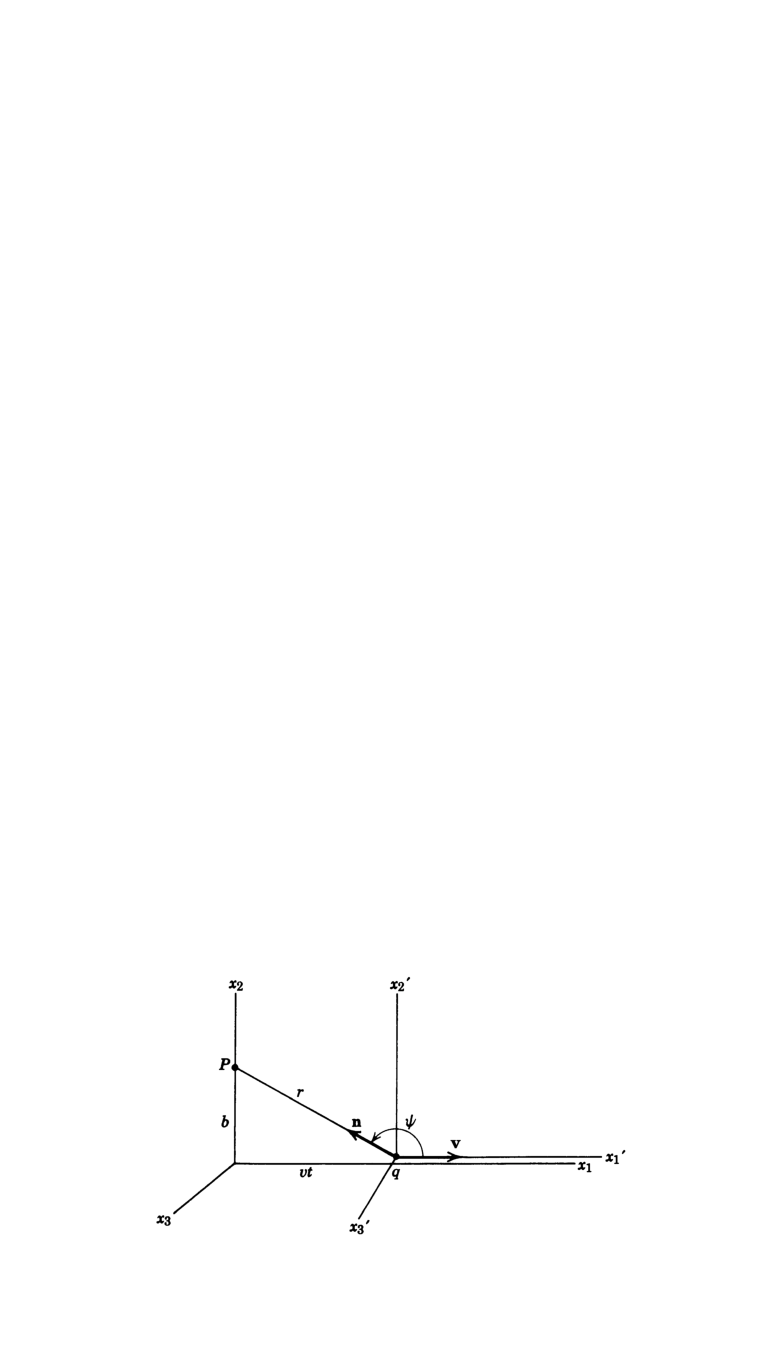
\includegraphics{11-8}
\caption{(Jackson Fig.~11.8) Particle of charge $q$ moving at constant velocity $\vv$ passes an observation point $P$ at impact parameter $b$.}
\label{11.8}
\end{figure}

\begin{problem} \label{2.a}
	For the geometry of Fig.~\ref{11.8} the coordinates of $P$ and $q$ at a common time in $K$ can be written $\xap = (ct, \vbb)$, $\xaq = (ct, \vv t)$, with $\vbb \vdot \vv = 0$.  By considering the general form of $\Fab$ in the rest frame of the charge, show that
	\beqn \label{show2.a}
		\Fab = \frac{q}{c} \frac{\Xa \Ub - \Xb \Ua}{[(\Usa \Xa / c)^2 - \Xsa \Xa]^{3/2}}.
	\eeqn
	Verify that this yields the expressions
	\begin{align} \label{fields}
		\Eq &= \Eq' = -\frac{q \gam v t}{(b^2 + \gam^2 v^2 t^2)^{3/2}}, &
		\Ew &= \gam \Ew' = \frac{\gam q b}{(b^2 + \gam^2 v^2 t^2)^{3/2}}, &
		\Be &= \gam \bet \Ew' = \bet \Ew,
	\end{align}
	with all other components vanishing, in the inertial frame $K$.
\end{problem}


\newcommand{\Fmat}{\mqty[	0 & -\Eq & -\Ew & -\Ee \\
						\Eq & 0 & -\Be & \Bw \\
						\Ew & \Be & 0 & -\Bq \\
						\Ee & -\Bw & \Bq & 0 ]}
\newcommand{\Fpab}{{F'}^{\alp\bet}}
\newcommand{\rp}{{r'}}
\newcommand{\tLam}{\tilde{\Lam}}
\newcommand{\Lammat}{\mqty[\gam & \gam \beta & 0 & 0 \\	
						\gam \beta & \gam & 0 & 0 \\
						0 & 0 & 1 & 0 \\
						0 & 0 & 0 & 1 ]}

\begin{solution}
	From Jackson~(11.137),
	\beqn \label{F}
		\Fab = \Fmat,
	\eeqn
	and from the equation immediately preceding Jackson~(11.151),
	\begin{align*}
		\Eq' &= -\frac{q v t'}{\rp^3}, &
		\Ew' &= \frac{q b}{\rp^3}, &
		\Ee' &= 0, &
		\Bq' &= 0, &
		\Bw' &= 0, &
		\Be' &= 0,
	\end{align*}
	in the rest frame of the charge.  Here, $r' = \sqrt{b^2 + v^2 {t'}^2}$.  Then, in $K'$,
	\beqn \label{thing2.1b}
		\Fpab = \frac{q}{(b^2 + v^2 {t'}^2)^{3/2}}
			\mqty[0 & v t' & -b & 0 \\
				-v t' & 0 & 0 & 0 \\
				b & 0 & 0 & 0 \\
				0 & 0 & 0 & 0 ].
	\eeqn
	Now we will boost into the frame $K$.  From Jackson~(11.147), $F' = \Lam F \tLam$, although we need $F = \Lam F' \tLam$, where we boost in the direction opposite the particle's motion.  According to Jackson~(11.113), the Lorentz boost in the $-{\xsq}'$ direction is
	\beqn \label{Lam2}
		\Lam^\alp_\bet = \Lammat.
	\eeqn
	Then
	\begin{align*}
		\Fab &= \frac{q}{(b^2 + v^2 {t'}^2)^{3/2}} \Lammat
			\mqty[ 0 & v t' & -b & 0 \\
				-v t' & 0 & 0 & 0 \\
				b & 0 & 0 & 0 \\
				0 & 0 & 0 & 0 ]
			\Lammat \\
		&= \frac{q}{(b^2 + v^2 {t'}^2)^{3/2}}
			\mqty[ -\gam \bet v t' & \gam v t' & -\gam b & 0 \\
				-\gam v t' & \gam \bet v t' & -\gam \bet b & 0 \\
				b & 0 & 0 & 0 \\
				0 & 0 & 0 & 0 ]
			\Lammat
		= \frac{q}{(b^2 + v^2 {t'}^2)^{3/2}}
			\mqty[ 0 & v t' & -\gam b & 0 \\
				-v t' & 0 & -\gam \bet b & 0 \\
				\gam b & \gam \bet b & 0 & 0 \\
				0 & 0 & 0 & 1 ].
	\end{align*}
	Note that $\xsq = 0$, so from \refeq{lorentz}, $t' = \gam t$.  Finally,
	\beqn \label{thing2.1}
		\Fab = \frac{\gam q}{(b^2 + \gam^2 v^2 t^2)^{3/2}} 
			\mqty[0 & v t & -b & 0 \\
				-v t & 0 & -v b / c & 0 \\
				b & v b / c & 0 & 0 \\
				0 & 0 & 0 & 0 ],
	\eeqn
	
	Now we will begin from \refeq{show2.a} and find $\Fab$ directly in $K$.  In accordance with Fig.~\ref{11.8},
	\begin{align*}
		\Xa &= (0, \vbb - \vv t) = (0, -v t, b, 0), &
		\Ua &= \gam (c, \vv) = \gam (c, v, 0, 0),
	\end{align*}
	and so
	\beq
		\Xa \Ub - \Xb \Ua = \gam
			\mqty[ 0 & 0 & 0 & 0 \\
				-c v t & -v^2 t & 0 & 0 \\
				c b & v b & 0 & 0 \\
				0 & 0 & 0 & 0 ]
		- \gam
			\mqty[ 0 & -c v t & c b & 0 \\
				0 & -v^2 t & v b & 0 \\
				0 & 0 & 0 & 0 \\
				0 & 0 & 0 & 0 ]
		= \gam
			\mqty[0 & c v t & - c b & 0 \\
				-c v t & 0 & -v b & 0 \\
				c b & v b & 0 & 0 \\
				0 & 0 & 0 & 0 ].
	\eeq
	Additionally,
	\begin{align*}
		\Usa \Xa &= \gam \mqty[ c & -v & 0 & 0 ] \mqty[ 0 \\ -v t \\ b \\ 0 ]
		= \gam v^2 t, &
		\Xsa \Xa &= \mqty[ 0 & vt & -b & 0 ] \mqty[ 0 \\ -v t \\ b \\ 0 ]
		= -v^2 t^2 - b^2.
	\end{align*}
	Then, applying \refeq{show2.a},
	\beq
		\Fab = \frac{\gam q}{(\gam^2 v^4 t^2 / c^2 + v^2 t^2 + b^2)^{3/2}}
			\mqty[0 & v t & -b & 0 \\
				-v t & 0 & -v b / c & 0 \\
				b & v b / c & 0 & 0 \\
				0 & 0 & 0 & 0 ].
	\eeq
	Note that
	\beq
		v^2 t^2 + \frac{\gam^2 v^4 t^2}{c^2} = v^2 t^2 \left( 1 + \gam^2 \frac{v^2}{c^2} \right)
		= v^2 t^2 \left( 1 + \frac{\bet^2}{1 - \bet^2} \right)
		= v^2 t^2 \frac{1 - \bet^2 + \bet^2}{1 - \bet^2}
		= \gam^2 v^2 t^2,
	\eeq
	so we have again arrived at \refeq{thing2.1}.  Thus, we have proven \refeq{show2.a}.
	
	In addition, comparing \refeq{thing2.1} with \refeq{F}, we see that
	\begin{align*}
		\Eq &= -\frac{q \gam v t}{(b^2 + \gam^2 v^2 t^2)^{3/2}}, &
		\Ew &= \frac{\gam q b}{(b^2 + \gam^2 v^2 t^2)^{3/2}}, &
		\Be &= \frac{\gam \bet q b}{(b^2 + \gam^2 v^2 t^2)^{3/2}} = \bet \Ew.
	\end{align*}
	Comparing \refeq{thing2.1b} with \refeq{F} as well, and making the substitution $t' = \gam t$, yields
	\begin{align*}
		\Eq' &= -\frac{q \gam v t}{(b^2 + \gam^2 v^2 t^2)^{3/2}}, &
		\Ew' &= \frac{q b}{(b^2 + \gam^2 v^2 t^2)^{3/2}},
	\end{align*}
	so we have also verified \refeq{fields}.
\end{solution}


\newcommand{\xpap}{{x'}^\alp_p}
\newcommand{\xpaq}{{x'}^\alp_q}
\newcommand{\Ya}{Y^\alp}
\newcommand{\Ysa}{Y_\alp}
\newcommand{\Yb}{Y^\bet}
\newcommand{\Ypa}{{Y'}^\alp}

\begin{problem}
	Repeat the calculation, using as the starting point the common-time coordinates in the rest frame, $\xpap = (ct', \vbb - \vv t')$ and $\xpaq = (ct', 0)$.  Show that
	\beqn \label{show2.b}
		\Fab = \frac{q}{c} \frac{\Ya \Ub - \Yb \Ua}{(- \Ysa \Ya)^{3/2}},
	\eeqn
	where $\Ypa = \xpap - \xpaq$.  Verify that the fields are the same as in \ref{2.a}.  Note that to obtain the results of \refeq{fields} it is necessary to use the time $t$ of the observation point $P$ in $K$ as the time parameter.
\end{problem}

\newcommand{\Ypsa}{{Y'}_\alp}
\newcommand{\Ypb}{{Y'}^\bet}
\newcommand{\Upa}{{U'}^\alp}
\newcommand{\Upb}{{U'}^\bet}
\newcommand{\voo}{\mathbf{0}}
\newcommand{\tp}{{t'}}

\begin{solution}
	Firstly, note that
	\begin{align*}
		\Ypa &= (0, \vbb - \vv t') = (0, -v t', b, 0), &
		\Upa &= (c, \voo) = (c, 0, 0, 0),
	\end{align*}
	Then
	\beq
		\Ypa \Upb - \Ypb \Upa = c
			\mqty[ 0 & 0 & 0 & 0 \\
				-v t' & 0 & 0 & 0 \\
				b & 0 & 0 & 0 \\
				0 & 0 & 0 & 0 ]
		- c
			\mqty[ 0 & -v t' & b & 0 \\
				0 & 0 & 0 & 0 \\
				0 & 0 & 0 & 0 \\
				0 & 0 & 0 & 0 ]
		= c
			\mqty[ 0 & v t' & -b & 0 \\
				-v t' & 0 & 0 & 0 \\
				b & 0 & 0 & 0 \\
				0 & 0 & 0 & 0 ],
	\eeq
	and
	\beq
		\Ypsa \Ypa = \mqty[ 0 & v t' & -b & 0 ] \mqty[ 0 \\ -v t' \\ b \\ 0 ] = -v^2 \tp^2 - b^2,
	\eeq
	so, from \refeq{show2.b}, in $K'$ we have
	\beq
		\Fpab = \frac{q}{(b^2 + v^2 \tp^2)^{3/2}}
			\mqty[ 0 & v t' & -b & 0 \\
				-v t' & 0 & 0 & 0 \\
				b & 0 & 0 & 0 \\
				0 & 0 & 0 & 0 ],
	\eeq
	which is identical to \refeq{thing2.1b}.  We know that boosting into $K$ yields \refeq{thing2.1}.
	
	Now we will find $\Fab$ directly in $K$ by boosting $\Ypa$ and $\Upa$.  From Jackson~(11.84), $x' = \Lam x$, and we once again use $\Lam$ given by \refeq{Lam2} to perform $x = \Lam x'$.  We obtain
	\begin{align*}
		Y &= \Lam Y'
		= \Lammat \mqty[ 0 \\ -v t' \\ b \\ 0]
		= \mqty[ -\gam \bet v t' \\ -\gam v t' \\ b \\ 0 ], &
		U &= \Lam U'
		= \Lammat \mqty[ c \\ 0 \\ 0 \\ 0 ]
		= \gam c \mqty[ 1 \\ \bet \\ 0 \\ 0 ].
	\end{align*}
	Then
	\beq
		\Ya \Ub - \Yb \Ua = \gam c
			\mqty[ -\gam \bet v t' & -\gam \bet^2 v t' & 0 & 0 \\
				-\gam v t' & -\gam \bet v t' & 0 & 0 \\
				b & \bet b & 0 & 0 \\
				0 & 0 & 0 & 0 ]
			- \gam c
			\mqty[ -\gam \bet v t' & -\gam v t' & b & 0 \\
				-\gam \bet^2 v t' & -\gam \bet v t' & \bet b & 0 \\
				0 & 0 & 0 & 0 \\
				0 & 0 & 0 & 0 ]
		= c
			\mqty[ 0 & v t' & -\gam b & 0 \\
				-v t' & 0 & -\gam \bet b & 0 \\
				\gam b & \gam \bet b & 0 & 0 \\
				0 & 0 & 0 & 0 ],
	\eeq
	and
	\beq
		\Ysa \Ya = \mqty[ -\gam \bet v t' & \gam v t' & -b & 0] \mqty[ -\gam \bet v t' \\ -\gam v t' \\ b \\ 0 ]
		= \gam^2 \bet^2 v^2 \tp^2 - \gam^2 v^2 \tp^2 - b^2
		= -v^2 \tp^2 - b^2.
	\eeq
	Making these substitutions into \refeq{show2.b}, and using $t' = \gam t$
	\beq
		\Fab = \frac{q}{(b^2 + v^2 \tp^2)^{3/2}}
			\mqty[ 0 & v t' & -\gam b & 0 \\
				-v t' & 0 & -\gam v b / c & 0 \\
				\gam b & \gam v b / c & 0 & 0 \\
				0 & 0 & 0 & 0 ]
		= \frac{\gam q}{(b^2 + \gam^2 v^2 t^2)^{3/2}}
			\mqty[ 0 & v t & -b & 0 \\
				-v t & 0 & -v b / c & 0 \\
				b & v b / c & 0 & 0 \\
				0 & 0 & 0 & 0 ],
	\eeq
	which is identical to \refeq{thing2.1}, and therefore gives the fields from \refeq{fields} as in \ref{2.a}.  Thus, we have proven \refeq{show2.b}. \qed
\end{solution}


\newcommand{\Za}{Z^\alp}
\newcommand{\Zsa}{Z_\alp}
\newcommand{\Zb}{Z^\bet}
\newcommand{\vbet}{\boldsymbol{\beta}}

\begin{problem}
	Finally, consider the coordinate $\xap = (ct, \vbb)$ and the ``retarded-time'' coordinate $\xaq = [ct - R, \vbet(ct - R)]$ where $R$ is the distance between $P$ and $q$ at the retarded time.  Define the difference as $\Za = [R, \vbb - \vbet(ct - R)]$.  Show that in terms of $\Za$ and $\Ua$ the field is
	\beqn \label{show2.c}
		\Fab = \frac{q}{c} \frac{\Za \Ub - \Zb \Ua}{(\Usa \Za / c)^3}.
	\eeqn
	\vfix
\end{problem}

\begin{solution}
	Referring to Fig~\ref{11.8},
	\begin{align*}
		\Za &= (R, \vbb - \vv t + \vv R / c) = [R, -v (t - R / c), b, 0], &
		\Ua &= \gam (c, \vv) = \gam (c, v, 0, 0).
	\end{align*}
	Then
	\begin{align*}
		\Za\Ub - \Zb \Ua &= \gam
			\mqty[c R & R v & 0 & 0 \\
				-v (c t - R) & -v^2 (t - R / c) & 0 & 0 \\
				c b & b v & 0 & 0 \\
				0 & 0 & 0 & 0 ]
			- \gam
			\mqty[ c R & -v (c t - R) & c b & 0 \\
				R v & -v^2 (t - R / c) & b v & 0 \\
				0 & 0 & 0 & 0 \\
				0 & 0 & 0 & 0 ] \\
		&= \gam c
			\mqty[0 & v t & -b & 0 \\
				-v t & 0 & -v b / c & 0 \\
				b & v b / c & 0 & 0 \\
				0 & 0 & 0 & 0 ],
	\end{align*}
	and
	\beq
		\Usa \Za = \gam \mqty[ c & -v & 0 & 0 ] \mqty[ R \\ -v (t - R / c) \\ b \\ 0 ]
		= \gam cR + \gam v^2(t - R/c),
	\eeq
	so
	\beq
		\frac{\Usa \Za}{c} = \gam R + \gam \bet^2 c t - \gam \bet^2 R
		= (1 - \bet^2) \gam R + \gam \bet^2 c t
		= \frac{R}{\gam} + \gam \bet^2 c t.
	\eeq
	
	Note that $\xap$ and $\xaq$, as they are defined here, have lightlike separation.  Then
	\beq
		0 = \Zsa \Za
		= \mqty[ R & v (t - R / c) & -b & 0 ] \mqty[ R \\ -v (t - R / c) \\ b \\ 0 ]
		= R^2 - v^2 (t - R / c)^2 - b^2,
	\eeq
	which implies
	\beq
		R^2 = b^2 + v^2 (t - R / c)^2.
	\eeq
	This is corroborated by the geometry of Fig.~\ref{11.8}.  Then, referring to the denominator of \refeq{thing2.1}, we find
	\begin{align*}
		b^2 + \gam^2 v^2 t^2 &= R^2 - v^2 (t - R / c)^2 + \gam^2 v^2 t^2
		= R^2 - \bet^2  (c^2 t^2 - 2 R c t + R^2) + \gam^2 \bet^2 c^2 t^2 \\
		&= (1 - \bet^2) R^2 + 2 R \bet^2 c t + (\gam^2 - 1) \bet^2 c^2 t^2
		= \frac{R^2}{\gam^2} + 2 R \bet^2 c t + \gam^2 \bet^4 c^2 t^2
		= \left( \frac{R}{\gam} + \gam \bet^2 c t \right)^2 \\
		&= \left( \frac{\Usa \Za}{c} \right)^2.
	\end{align*}
	Thus, we have found
	\beq
		\Fab = \frac{\gam q}{(b^2 + \gam^2 v^2 t^2)^{3/2}}
			\mqty[0 & v t & -b & 0 \\
				-v t & 0 & -v b / c & 0 \\
				b & v b / c & 0 & 0 \\
				0 & 0 & 0 & 0 ],
	\eeq
	which is identical to \refeq{thing2.1}.  Thus, we have proven \refeq{show2.c}. \qed
\end{solution}